\label{sec:resultados}

Este capítulo apresenta o artefato e sua avaliação. A Seção~\ref{sec:res-requisitos} traz os requisitos e a matriz de rastreabilidade. As Seções~\ref{sec:res-visao} a \ref{sec:res-componentes} descrevem a arquitetura. As Seções~\ref{sec:res-criterios} a \ref{sec:res-dados} detalham os critérios clínicos, a integração com a RNDS e a proteção de dados. A Seção~\ref{sec:res-decisoes} registra as decisões arquiteturais, a Seção~\ref{sec:res-avaliacao} apresenta os resultados da avaliação analítica e as Seções~\ref{sec:res-discussao} e \ref{sec:res-limitacoes} discutem os resultados e seus limites.

\subsecao{Requisitos e matriz de rastreabilidade}
\label{sec:res-requisitos}

A revisão produziu 19 requisitos: 10 funcionais e 9 não funcionais. A Tabela~\ref{tab:rastreabilidade} vincula cada requisito à fonte que o originou, ao risco que ele endereça e aos componentes responsáveis. Os componentes citados são descritos nas Seções~\ref{sec:res-visao} e \ref{sec:res-componentes}.

{\footnotesize
\begin{longtable}{L{0.9cm} L{4.3cm} L{1.8cm} L{3.0cm} L{3.4cm}}
\caption{Matriz de rastreabilidade entre fontes, requisitos, riscos e componentes}\label{tab:rastreabilidade}\\
\toprule
\textbf{ID} & \textbf{Requisito} & \textbf{Fonte} & \textbf{Risco endereçado} & \textbf{Componentes} \\
\midrule
\endfirsthead
\toprule
\textbf{ID} & \textbf{Requisito} & \textbf{Fonte} & \textbf{Risco endereçado} & \textbf{Componentes} \\
\midrule
\endhead
\midrule
\multicolumn{5}{r}{\textit{continua na próxima página}}\\
\endfoot
\bottomrule
\endlastfoot
RF1 & Restringir o canal a pacientes com classificação verde ou azul registrada em triagem presencial e que atendam aos critérios de elegibilidade & \cite{stormversloot2014, sorznechay2025} & Uso do canal remoto por paciente de maior gravidade & Estação de enfermagem, Gestão de Atendimentos, Aplicação do totem \\
RF2 & Registrar a classificação e os sinais vitais e disponibilizá-los ao médico remoto & \cite{portaria234, rcp2017news2} & Perda de contexto entre a triagem e a teleconsulta & Estação de enfermagem, Prontuário Local, Estação do médico \\
RF3 & Identificar o paciente por CNS ou CPF & \cite{portaria234, rndsig} & Registro clínico vinculado a indivíduo errado & Aplicação do totem, Gestão de Atendimentos, Gateway FHIR \\
RF4 & Coletar e registrar o consentimento explícito para o atendimento remoto, com confirmação pelo médico & \cite{cfm2314, lei14510} & Ato médico sem autorização documentada & Aplicação do totem, Prontuário Local, Estação do médico \\
RF5 & Permitir a recusa e o retorno ao atendimento presencial a qualquer momento, com registro do motivo & \cite{lei14510, cfm2314} & Restrição indevida da autonomia do paciente ou do médico & Aplicação do totem, Gestão de Atendimentos, Estação do médico \\
RF6 & Agendar reavaliações, receber sinais vitais e chamadas do totem, alertar a enfermagem e suspender a teleconsulta em caso de piora & \cite{rcp2017news2, stormversloot2014} & Agravamento não detectado durante a espera & Reavaliação e Alertas, Estação de enfermagem, Aplicação do totem, Notificações \\
RF7 & Coletar a queixa de forma estruturada, por toque ou voz & \cite{portaria234, joseph2023} & Queixa incompleta ou ilegível para o médico & Aplicação do totem, Prontuário Local \\
RF8 & Realizar a teleconsulta por áudio e vídeo, com distribuição dos pacientes entre os médicos disponíveis & \cite{cfm2314, portaria3691} & Espera sem atendimento ou sessão de baixa qualidade & Plataforma de teleconsulta, Estação do médico, Gestão de Atendimentos \\
RF9 & Registrar conduta, desfecho e documentos com assinatura digital ICP-Brasil e entregar as orientações ao paciente & \cite{cfm2314, portaria234} & Documento sem validade ou orientação não recebida & Estação do médico, Prontuário Local, Notificações \\
RF10 & Consultar o histórico disponível e enviar o RAC à RNDS ao fim do atendimento & \cite{portaria234, portaria3691, rndsconector} & Atendimento desconectado da rede de atenção & Gateway FHIR, Fila de mensagens \\
\midrule
RNF1 & Vedar triagem, diagnóstico e conduta automatizados; o totem é apenas canal pós-triagem (adequação funcional) & \cite{dickson2022, joseph2023} & Subclassificação de risco por instrumento não validado & Gestão de Atendimentos, Aplicação do totem \\
RNF2 & Montar os registros em HL7 FHIR R4 com os perfis e terminologias nacionais e validá-los antes do envio (compatibilidade) & \cite{rndsig, portaria234, hl7fhirr4} & Rejeição do documento e ausência de registro na rede & Gateway FHIR \\
RNF3 & Tratar os dados sob a hipótese de tutela da saúde, com minimização, retenção definida e auditoria imutável (segurança) & \cite{lgpd2018, leme2020, lei13787} & Dado sensível tratado sem base legal ou sem rastro & Auditoria, Registro de auditoria, Banco de dados, API Gateway, Aplicação do totem \\
RNF4 & Proteger a confidencialidade em ambiente público e a integridade física e lógica do totem (segurança) & \cite{lei14510, lgpd2018} & Exposição de dados a terceiros ou adulteração do dispositivo & Aplicação do totem \\
RNF5 & Manter o registro clínico diante de falhas de rede ou da RNDS, com reenvio e idempotência (confiabilidade) & \cite{rndserros, rndsconector} & Perda ou duplicação de registros clínicos & Gateway FHIR, Fila de mensagens, Notificações \\
RNF6 & Assegurar acessibilidade física e digital e atendimento assistido alternativo (usabilidade) & \cite{lbi2015, nbr9050, emag, wcag21, joseph2023} & Exclusão por deficiência ou baixa literacia digital & Aplicação do totem, Estação de enfermagem \\
RNF7 & Manter módulos de baixo acoplamento, com evolução independente (manutenibilidade) & \cite{goeg2018, jat2024} & Obsolescência diante de mudanças nos perfis nacionais & Gateway FHIR, Fila de mensagens, todos os serviços \\
RNF8 & Autenticar os profissionais e controlar o acesso por perfis (segurança) & \cite{lgpd2018, cfm2314} & Acesso indevido a dados clínicos & Autenticação e Autorização, API Gateway \\
RNF9 & Oferecer monitoramento operacional ao gestor com dados agregados, sem dados clínicos identificados (segurança) & \cite{lgpd2018, pearce2024} & Uso de dado clínico para finalidade diversa & Painel do gestor \\
\end{longtable}
}
\fonte{Elaboração própria.}

Dois requisitos merecem destaque. O RF1 e o RNF1 materializam a decisão central da proposta: o totem não classifica risco, e o uso do canal remoto depende de uma triagem presencial registrada e de critérios adicionais. O RNF2 traduz a observação de que adotar o FHIR não basta, e que a conformidade depende dos perfis e regras de envio da rede nacional.

\subsecao{Visão geral da solução}
\label{sec:res-visao}

A Figura~\ref{fig:fluxo}, apresentada no Capítulo~\ref{sec:introducao}, resume em cinco etapas o funcionamento da solução do ponto de vista de quem participa do atendimento. As seções seguintes detalham a arquitetura que sustenta esse fluxo.

A arquitetura que sustenta esse fluxo foi organizada em cinco camadas funcionais (Figura~\ref{fig:camadas}). As quatro primeiras têm responsabilidades sequenciais, do contato com o paciente até a integração externa. A quinta, de segurança, atravessa todas as outras.

\begin{figure}[H]
\centering
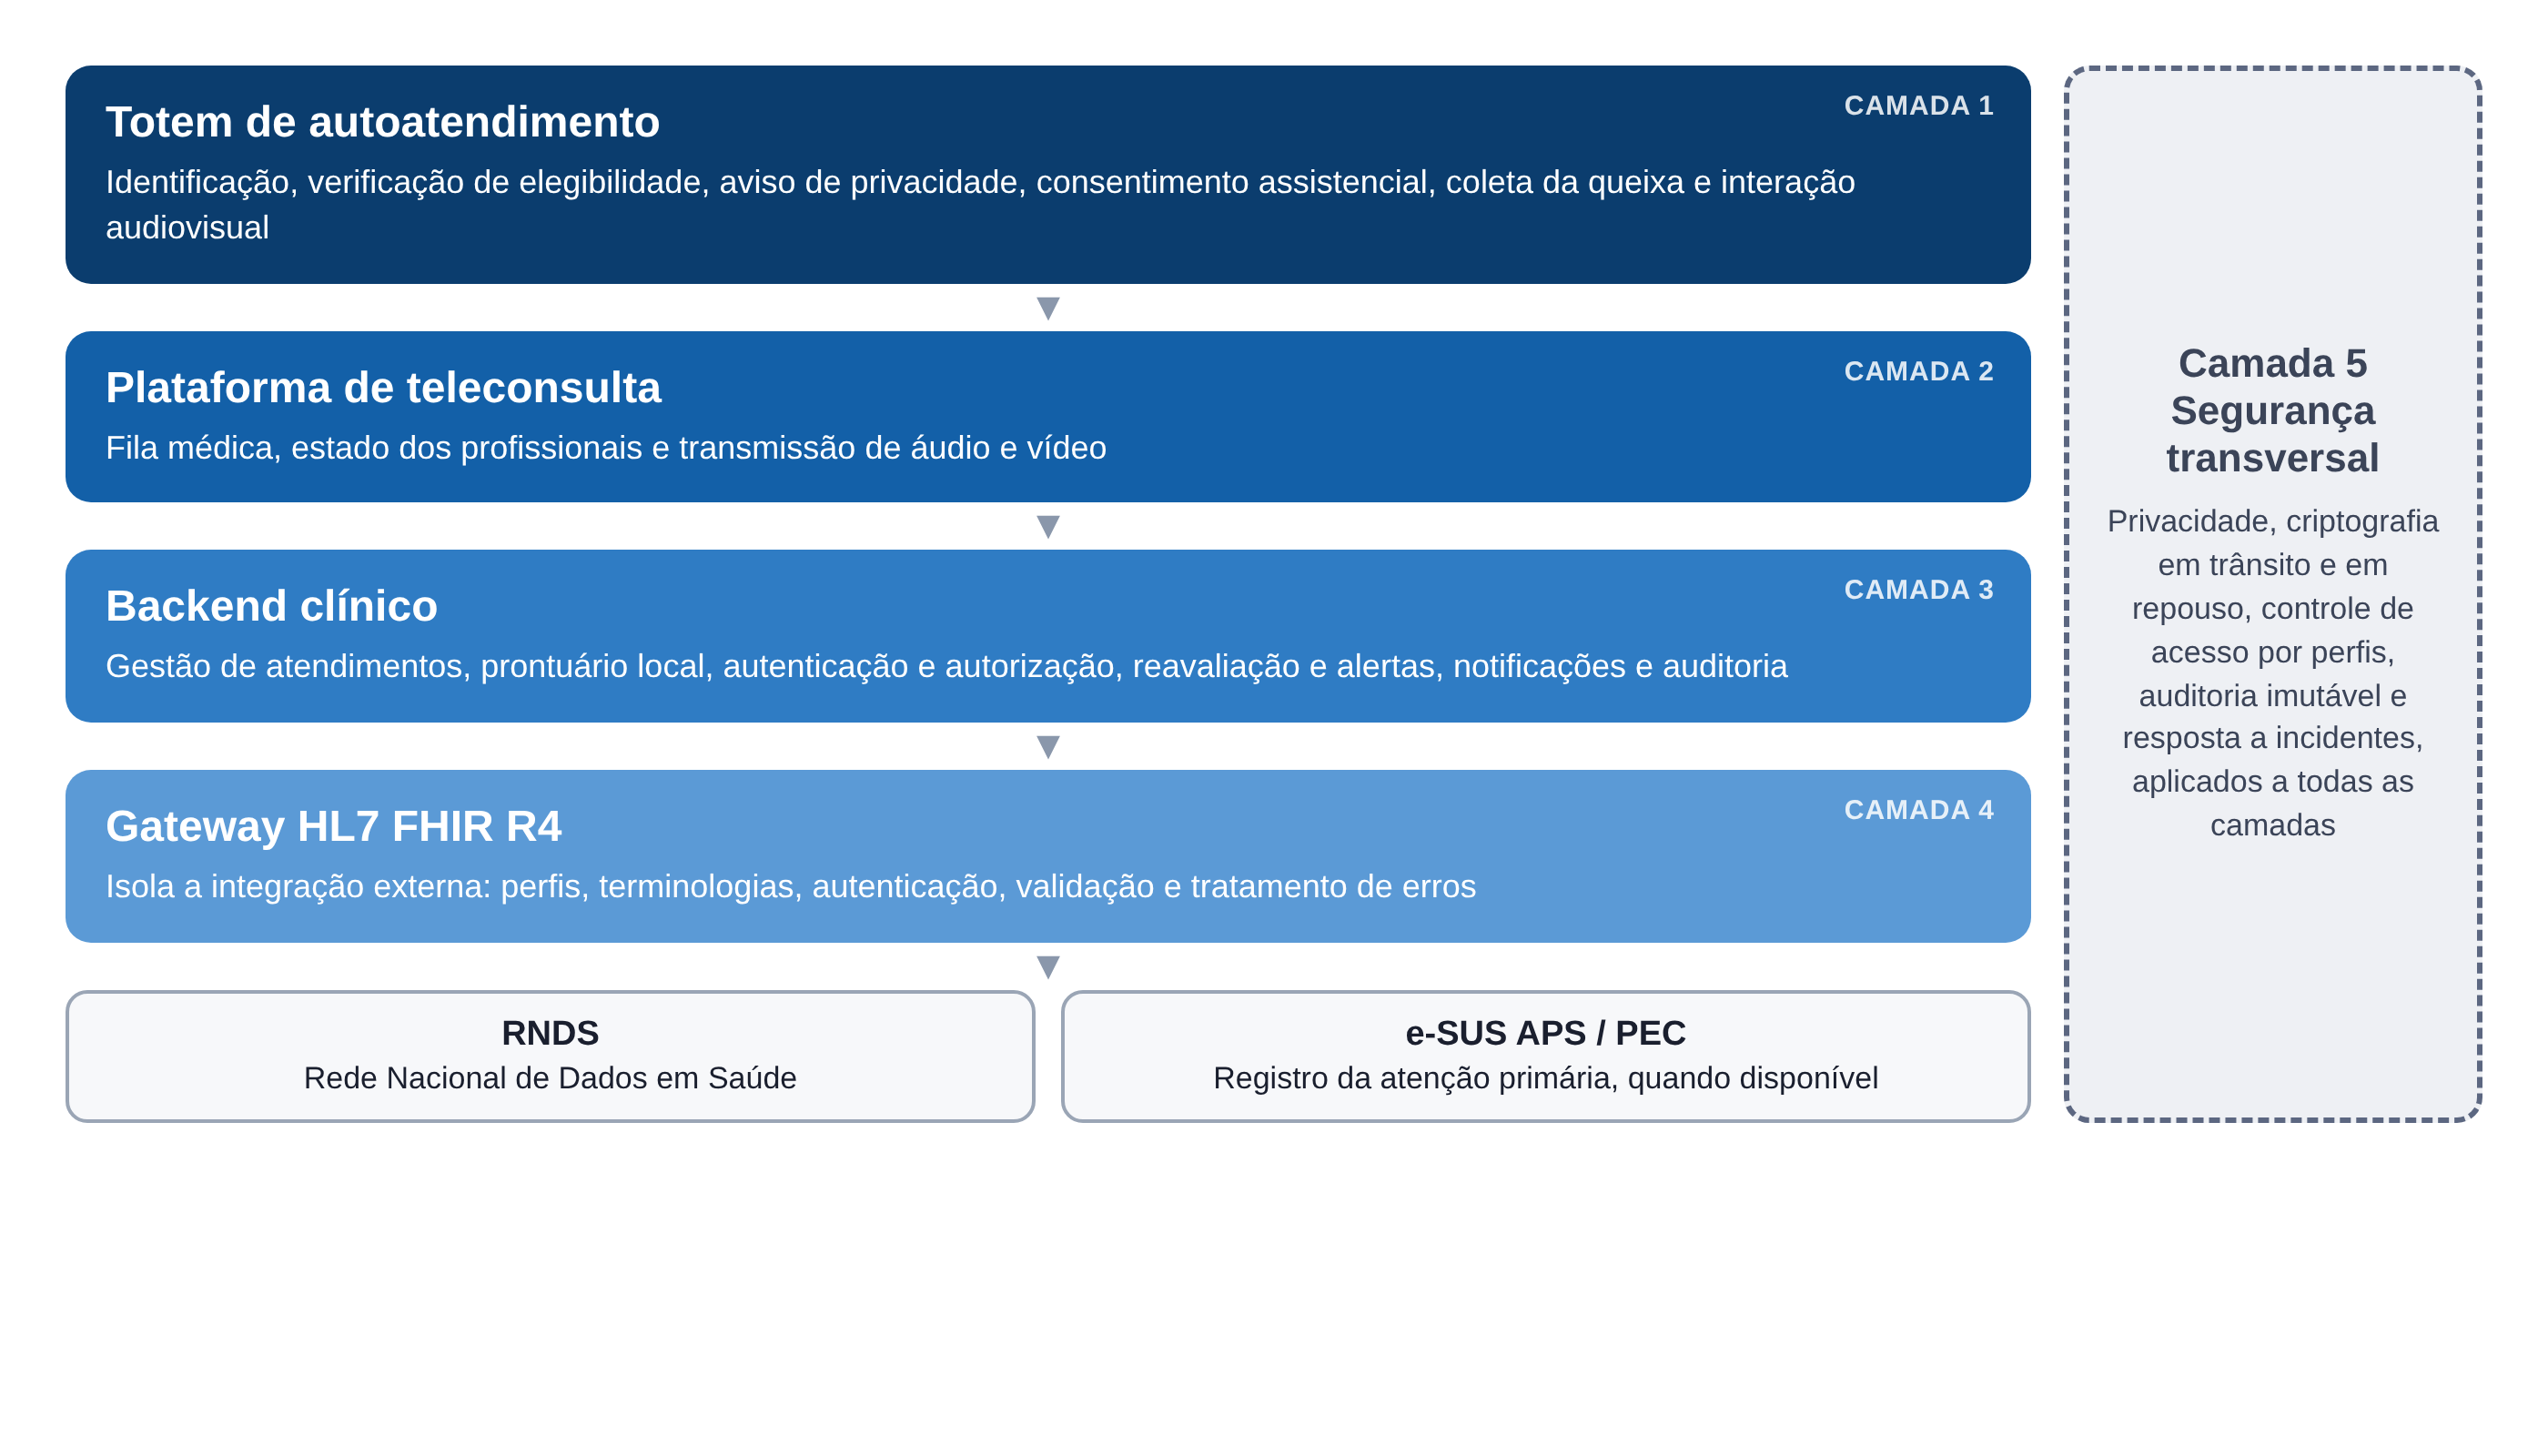
\includegraphics[width=0.92\textwidth]{figuras/camadas.png}
\caption{Camadas funcionais da arquitetura proposta}
\label{fig:camadas}
\fonte{Elaboração própria.}
\end{figure}

\begin{itemize}
    \item \textbf{Camada 1, totem de autoatendimento.} Concentra a identificação, a verificação de elegibilidade, o aviso de privacidade, o consentimento assistencial, a coleta estruturada da queixa e a interação audiovisual.
    \item \textbf{Camada 2, plataforma de teleconsulta.} Gerencia a fila médica, o estado dos profissionais e a transmissão de áudio e vídeo.
    \item \textbf{Camada 3, backend clínico.} Coordena o ciclo do atendimento pelos serviços de gestão de atendimentos, prontuário local, autenticação e autorização, reavaliação e alertas, notificações e auditoria.
    \item \textbf{Camada 4, gateway FHIR.} Isola a integração com a RNDS e com o e-SUS APS, concentrando perfis, terminologias, autenticação, validação e tratamento de erros.
    \item \textbf{Camada 5, segurança transversal.} Aplica privacidade, criptografia em trânsito e em repouso, controle de acesso por perfis, auditoria imutável e resposta a incidentes.
\end{itemize}

\subsubsecao{Contexto}

O diagrama de contexto (Figura~\ref{fig:contexto}) mostra o sistema, seus quatro tipos de usuário e os sistemas externos. O paciente interage com o totem. A enfermagem registra a triagem, os sinais vitais e as reavaliações. O médico remoto conduz a teleconsulta e registra o desfecho. O gestor da unidade acompanha a operação e recebe alertas. Entre os sistemas externos, a RNDS é obrigatória, o registro da atenção primária é consultado quando disponível, e um serviço de mensagens entrega as orientações ao paciente.

\begin{figure}[H]
\centering
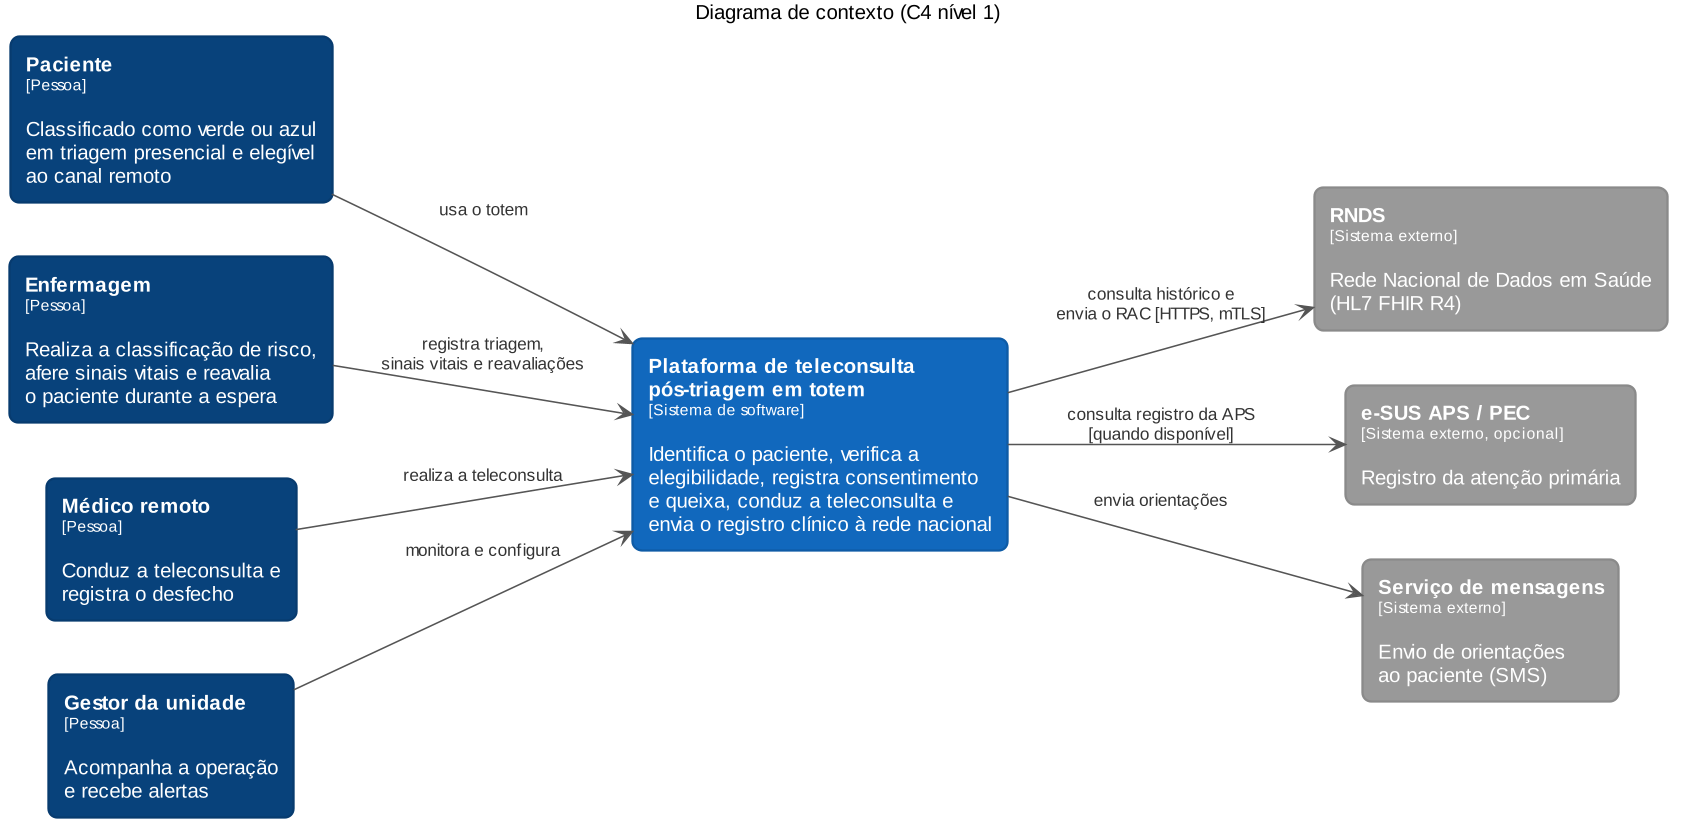
\includegraphics[width=\textwidth]{figuras/c4-contexto.png}
\caption{Diagrama de contexto (C4 nível 1)}
\label{fig:contexto}
\fonte{Elaboração própria com a ferramenta PlantUML.}
\end{figure}

\subsubsecao{Contêineres}

O diagrama de contêineres (Figura~\ref{fig:conteineres}) mostra as aplicações e armazenamentos que compõem o sistema. Há quatro aplicações de interface: a do totem, executada como aplicação web progressiva em modo quiosque, e as estações de enfermagem e do médico e o painel do gestor, executados em navegador. Todas acessam o backend por um API Gateway, que centraliza autenticação, roteamento e limitação de acesso. A mídia da teleconsulta trafega entre o totem e a estação do médico pela plataforma de teleconsulta, que combina um serviço de sinalização e um servidor de mídia. O backend publica eventos em uma fila de mensagens, que aciona o gateway FHIR para o envio do RAC sem bloquear o atendimento.

\begin{figure}[H]
\centering
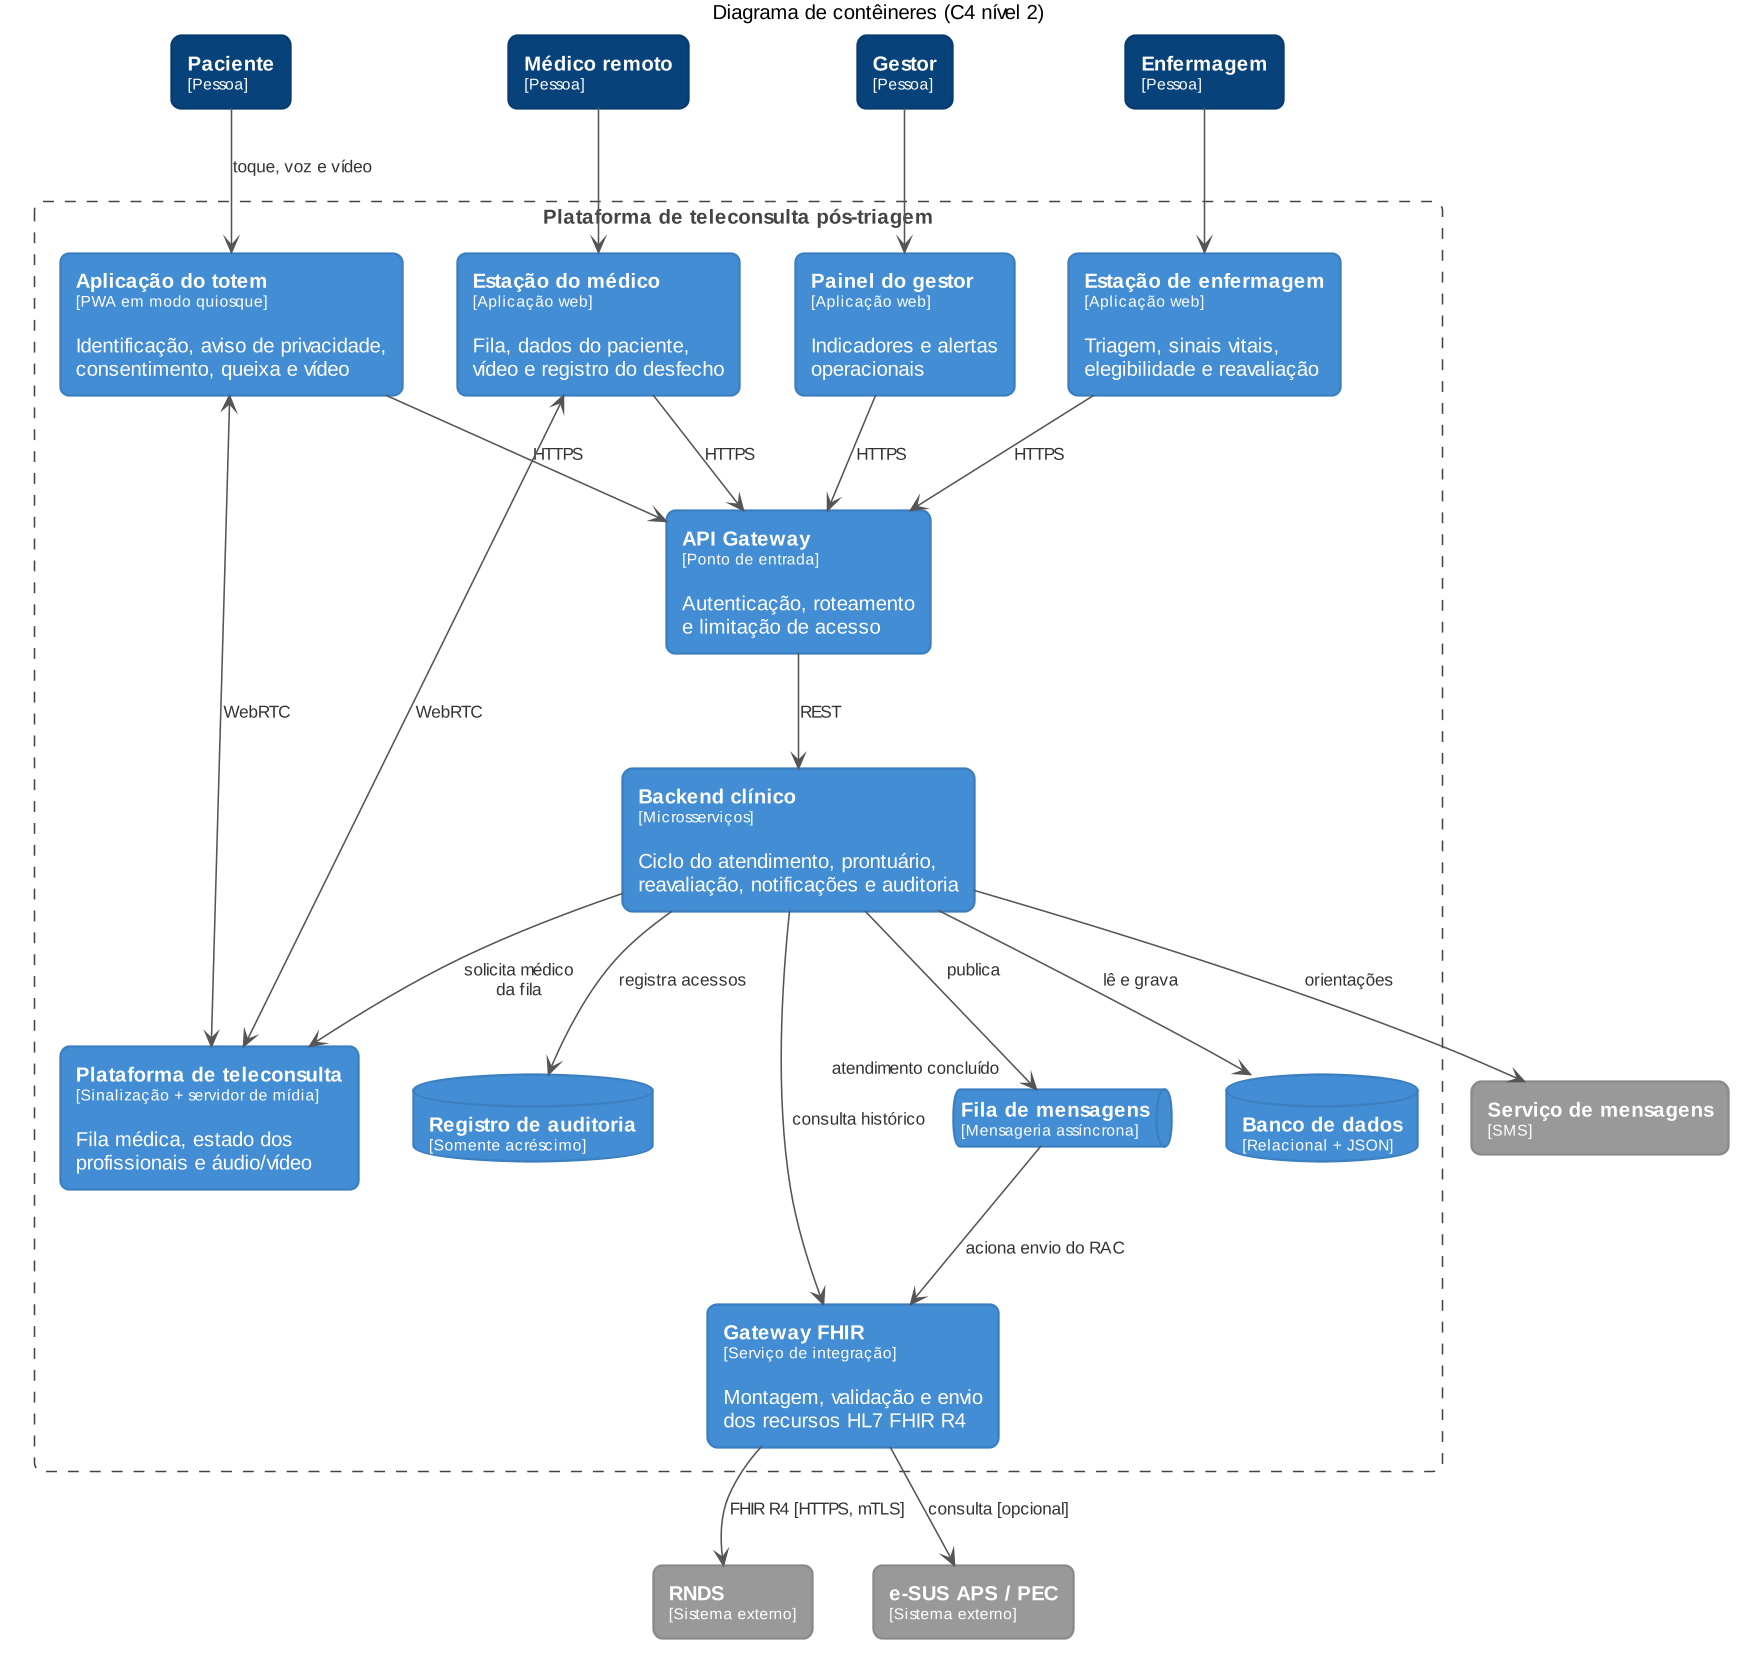
\includegraphics[width=0.95\textwidth]{figuras/c4-conteineres.png}
\caption{Diagrama de contêineres (C4 nível 2)}
\label{fig:conteineres}
\fonte{Elaboração própria com a ferramenta PlantUML.}
\end{figure}

\subsubsecao{Fluxo de atendimento}

As Figuras~\ref{fig:sequencia1} e \ref{fig:sequencia2} detalham, em diagrama de sequência, o fluxo da Figura~\ref{fig:fluxo}, dividido em duas partes para preservar a legibilidade. Três pontos do fluxo foram desenhados como barreiras de segurança. O primeiro é a verificação, no backend, de que existe uma triagem registrada e de que o paciente atende aos critérios e está dentro do prazo de espera, antes que o totem libere qualquer funcionalidade. O segundo é a repetição da reavaliação durante a espera, com suspensão da teleconsulta em caso de piora. O terceiro é o tratamento das falhas no envio do RAC, que nunca bloqueia o encerramento do atendimento.

\begin{figure}[H]
\centering
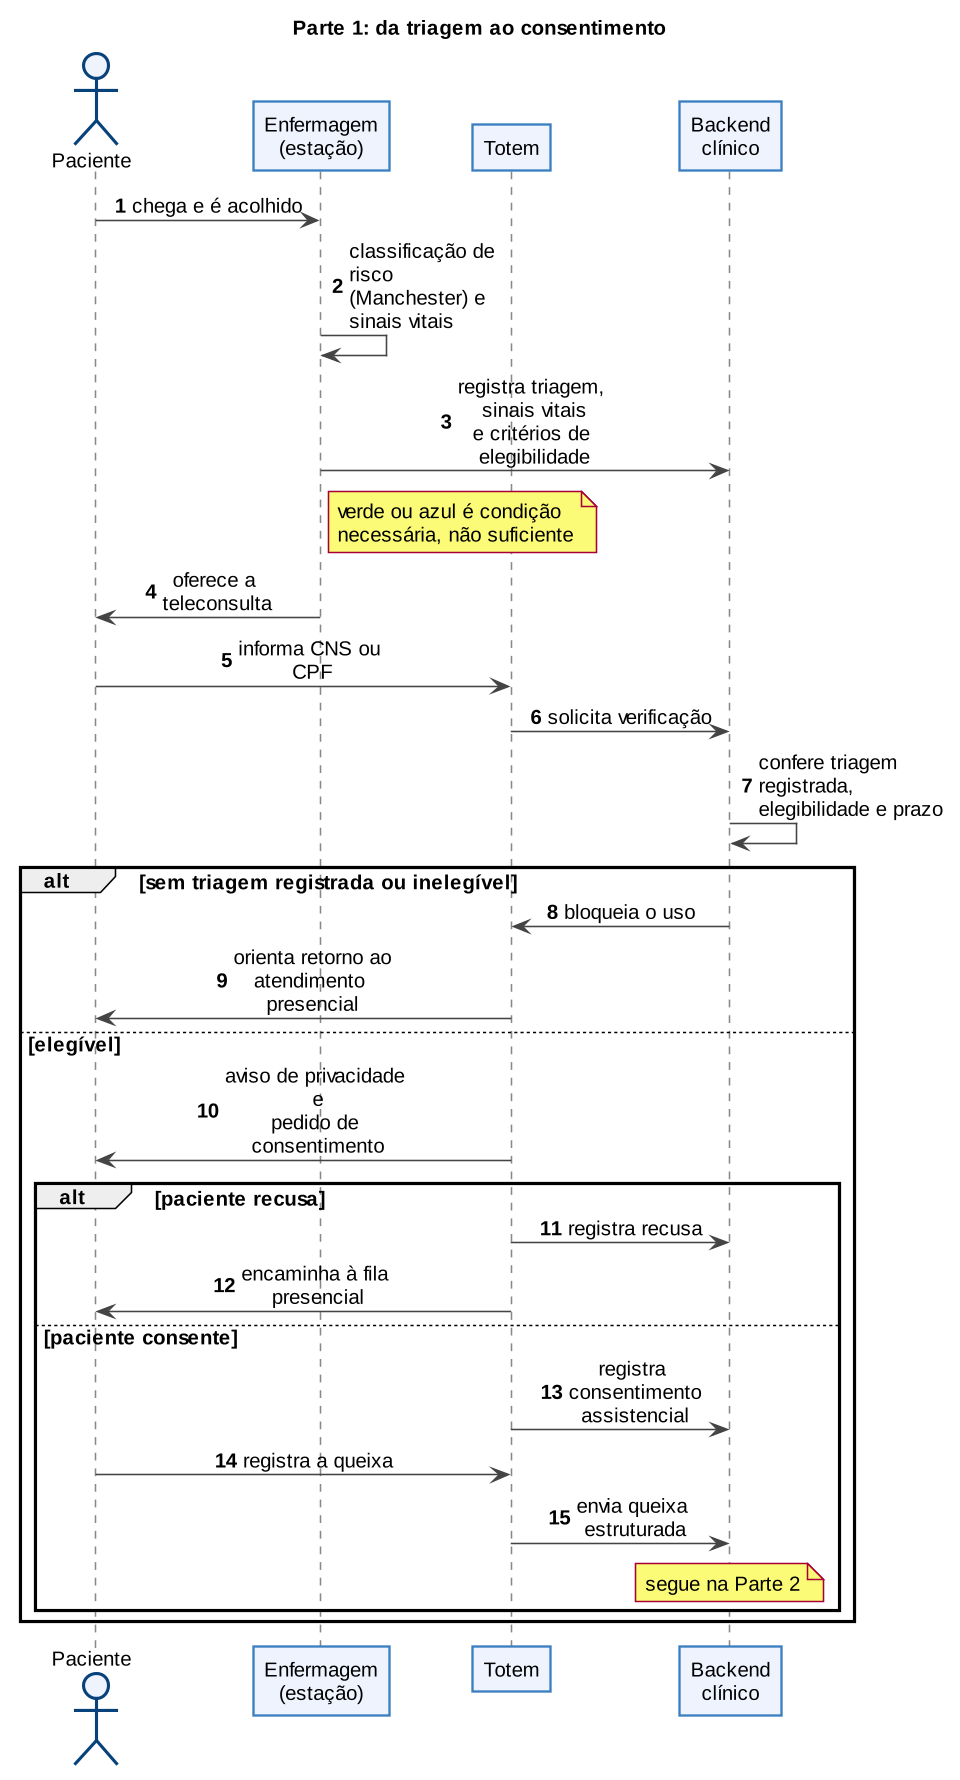
\includegraphics[height=0.72\textheight,width=\textwidth,keepaspectratio]{figuras/sequencia-1.png}
\caption{Fluxo de atendimento, parte 1: da triagem ao consentimento}
\label{fig:sequencia1}
\fonte{Elaboração própria com a ferramenta PlantUML.}
\end{figure}

\begin{figure}[H]
\centering
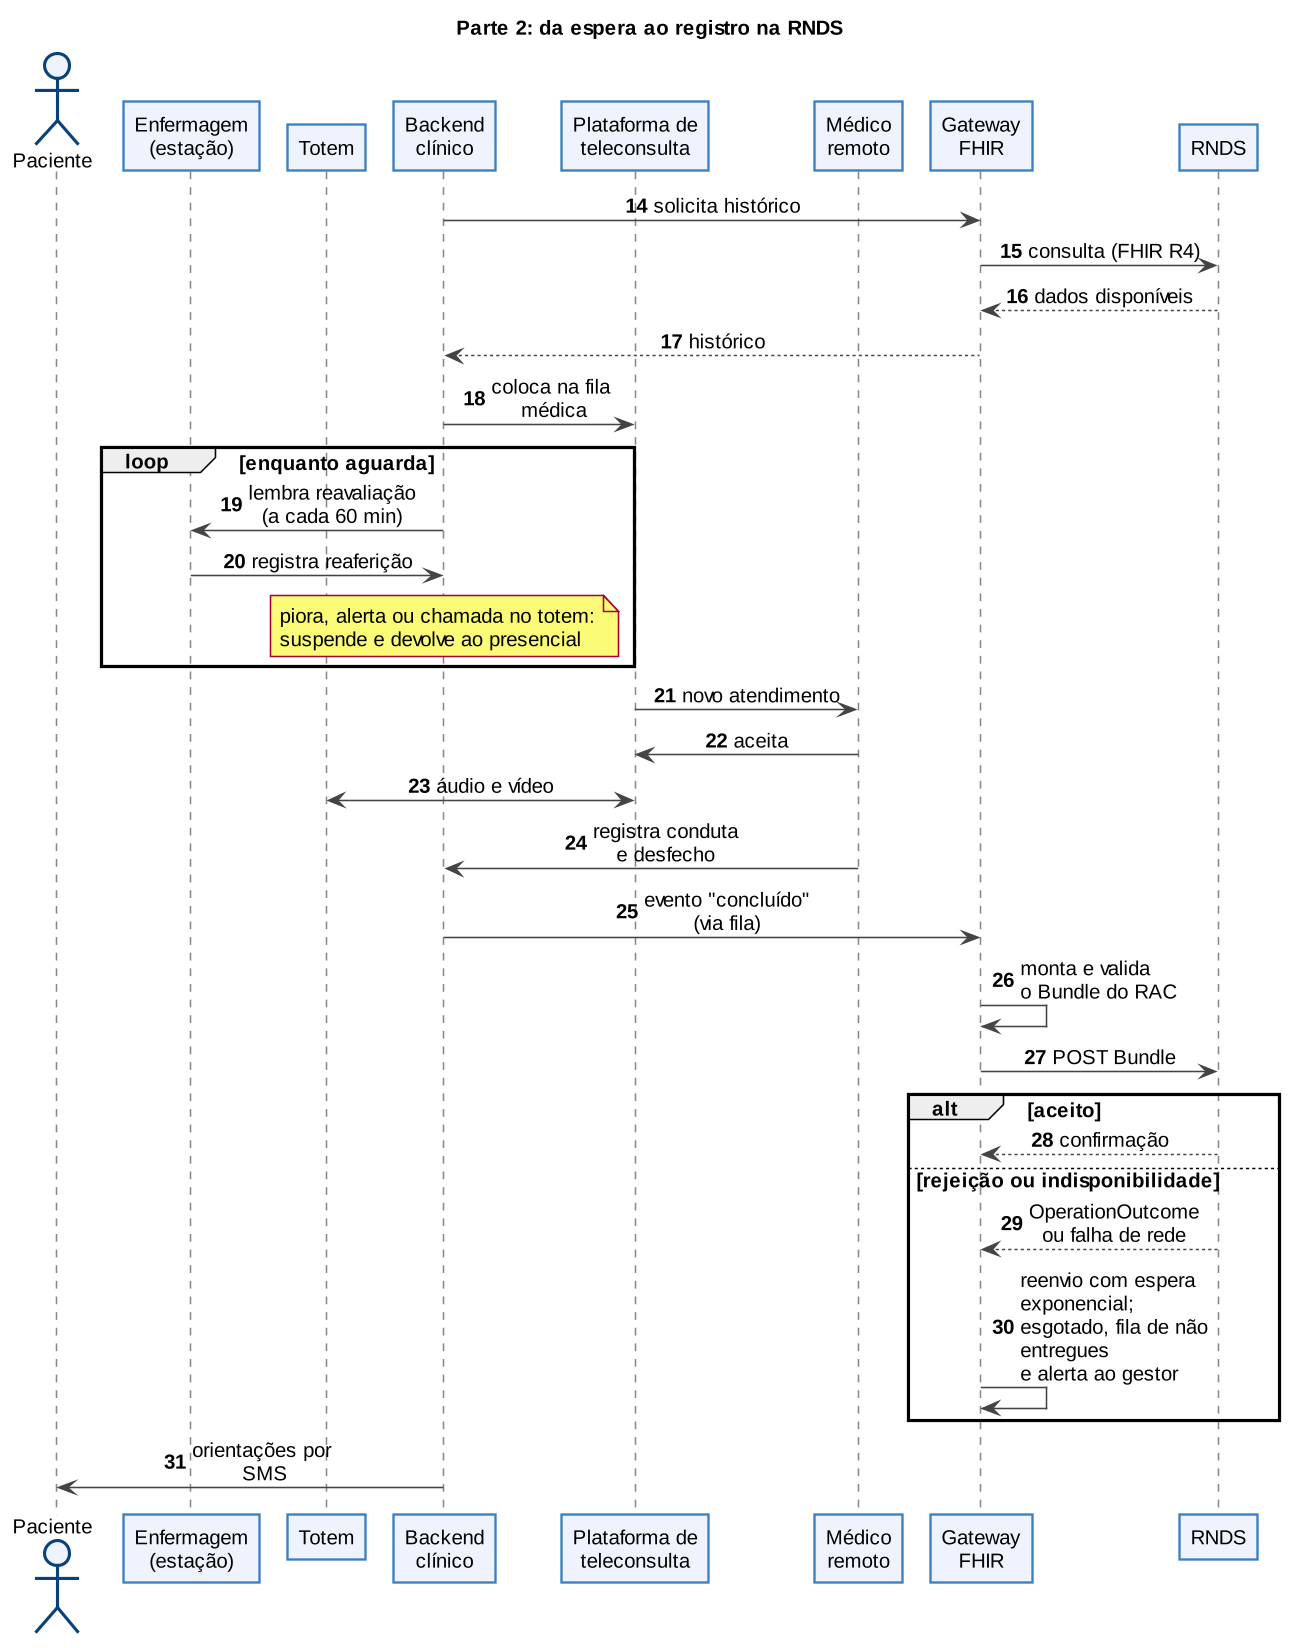
\includegraphics[height=0.72\textheight,width=\textwidth,keepaspectratio]{figuras/sequencia-2.png}
\caption{Fluxo de atendimento, parte 2: da espera ao registro na RNDS}
\label{fig:sequencia2}
\fonte{Elaboração própria com a ferramenta PlantUML.}
\end{figure}

\subsecao{Componentes da arquitetura}
\label{sec:res-componentes}

\subsubsecao{Totem de autoatendimento}

O totem é um dispositivo dedicado, instalado na unidade, com tela sensível ao toque, câmera, microfone, saída de áudio com fone de ouvido, leitor para o cartão do SUS ou teclado para o CPF e conexão de rede. A escolha de um equipamento dedicado, em vez de dispositivos do próprio paciente, decorre da necessidade de um ambiente de hardware e software controlado, com superfície de ataque reduzida e gestão centralizada. A aplicação é executada em modo quiosque, com uma única aplicação em tela cheia, sem acesso ao sistema operacional ou a navegação livre, e não guarda dados clínicos localmente ao fim da sessão. Os controles de privacidade, segurança física e acessibilidade do totem estão na Seção~\ref{sec:res-dados}.

\subsubsecao{Plataforma de teleconsulta}

A plataforma é composta pelo serviço de sinalização, que estabelece as sessões, pelo servidor de mídia, que encaminha os fluxos de áudio e vídeo, e pelo gerenciador de fila, que distribui os pacientes entre os médicos disponíveis segundo o estado de cada profissional (disponível, em atendimento, indisponível) e eventuais restrições configuradas pelo gestor. A transmissão usa protocolos abertos de comunicação em tempo real executados no navegador, sem complementos instalados, o que mantém a independência de fornecedores. O tempo estimado de espera é exibido continuamente ao paciente.

\subsubsecao{Backend clínico}

O backend é formado por serviços independentes, cada um com responsabilidade delimitada (Figura~\ref{fig:componentes}):
\begin{itemize}
    \item \textbf{Gestão de Atendimentos}: controla o ciclo de vida do atendimento, aplica a regra de elegibilidade vinculada à triagem registrada, controla os prazos máximos de espera e solicita o médico à plataforma de teleconsulta;
    \item \textbf{Reavaliação e Alertas}: agenda as reavaliações de enfermagem, recebe as reaferições de sinais vitais e as chamadas feitas no totem, dispara alertas e suspende a teleconsulta, devolvendo o paciente ao fluxo presencial;
    \item \textbf{Prontuário Local}: guarda o registro clínico da unidade, o consentimento assistencial e o histórico consultado na RNDS, que funciona como \textit{cache} em caso de conectividade intermitente;
    \item \textbf{Autenticação e Autorização}: gerencia a identidade dos profissionais e o controle de acesso por perfis;
    \item \textbf{Notificações}: entrega as orientações ao paciente e os alertas à enfermagem e ao gestor;
    \item \textbf{Auditoria}: registra, de forma imutável, os acessos e as ações sobre dados de saúde, com usuário, data, hora, recurso e origem.
\end{itemize}

\begin{sidewaysfigure}
\centering
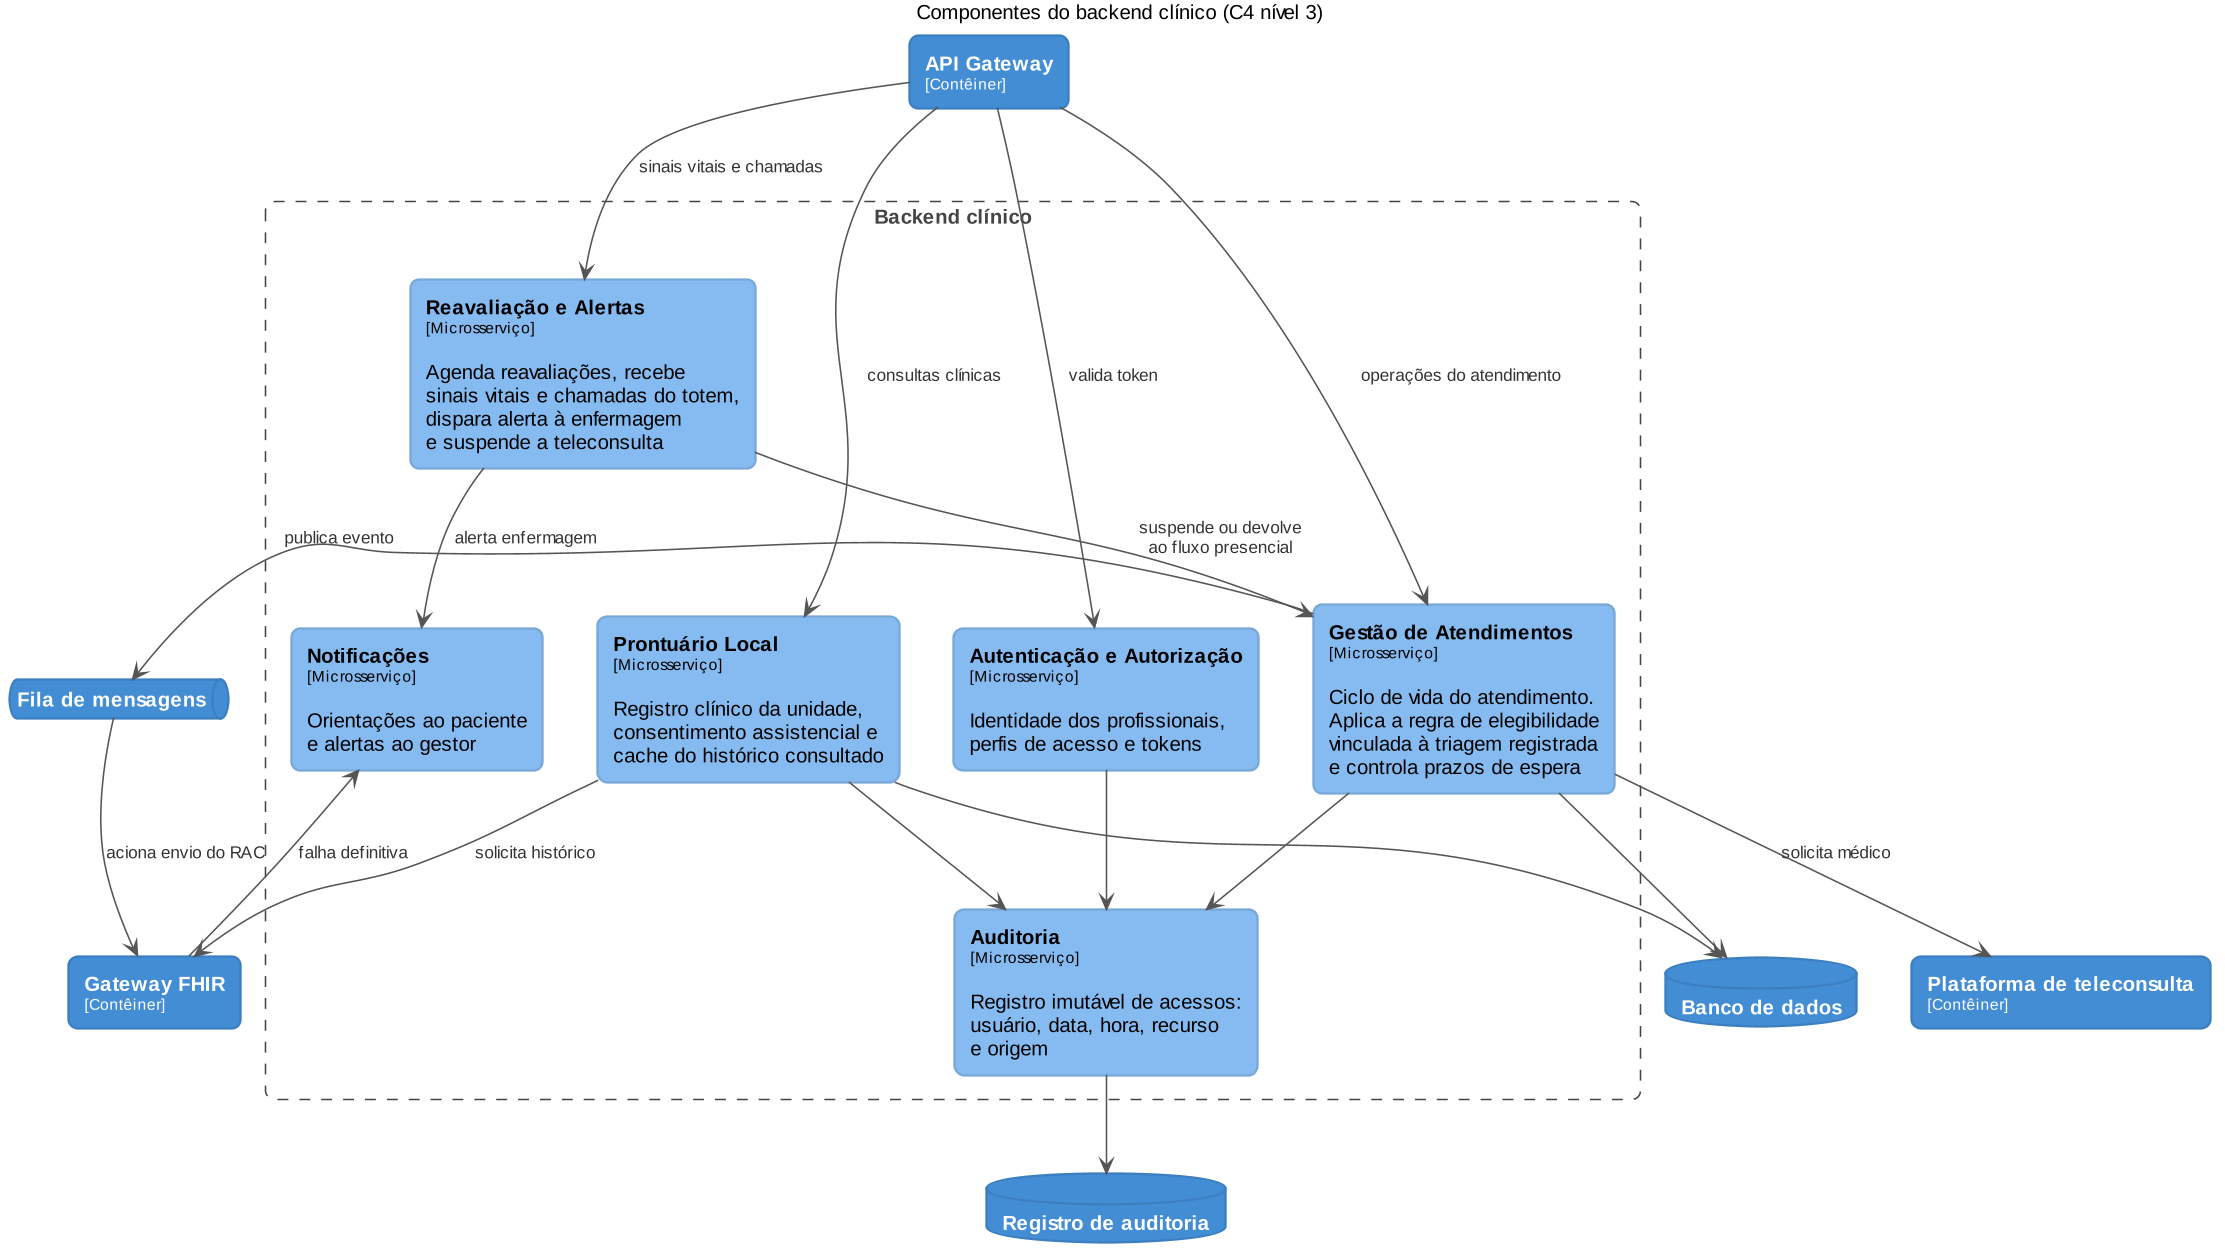
\includegraphics[width=\textheight]{figuras/c4-componentes.png}
\caption{Componentes do backend clínico (C4 nível 3)}
\label{fig:componentes}
\fonte{Elaboração própria com a ferramenta PlantUML.}
\end{sidewaysfigure}

A comunicação entre os serviços é síncrona, por interfaces REST, quando a operação precisa de resposta imediata, e assíncrona, por fila de mensagens, quando pode ser concluída depois, como o envio do RAC. A opção por serviços independentes e pela separação entre comunicação síncrona e assíncrona é discutida na Seção~\ref{sec:res-decisoes}.

\subsubsecao{Gateway FHIR}

O gateway concentra toda a comunicação com a RNDS e com o e-SUS APS. Ele monta os recursos FHIR a partir dos dados do atendimento, valida-os contra os perfis nacionais, obtém e renova o token de acesso, envia os documentos e interpreta as respostas. Como nenhum outro componente conhece os detalhes da rede nacional, uma mudança de perfil ou de regra de envio fica restrita a ele. A especificação está na Seção~\ref{sec:res-rnds}.

\subsubsecao{Segurança transversal}

A camada de segurança não é um componente isolado, mas um conjunto de controles aplicados em todas as camadas: criptografia em trânsito entre todos os componentes e com a RNDS; criptografia em repouso dos dados clínicos; autenticação dos profissionais e controle de acesso por perfis, em que o médico acessa apenas os pacientes que atende ou atendeu e o gestor acessa apenas dados agregados; auditoria imutável; e um processo formal de resposta a incidentes, com contenção e comunicação à autoridade nacional e ao titular, conforme o art. 48 da LGPD \cite{lgpd2018}.

\subsecao{Elegibilidade, reavaliação e retorno seguro}
\label{sec:res-criterios}

A classificação verde ou azul foi tratada como condição necessária, mas não suficiente, para o encaminhamento ao totem. Essa escolha segue o desenho do processo de encaminhamento estudado por Sorz-Nechay et al., em que a cor atribuída pela triagem era complementada por decisão médica e por critérios de exclusão \cite{sorznechay2025}. A Tabela~\ref{tab:criterios} apresenta os critérios propostos. Eles foram derivados da literatura e das normas, mas são uma proposta do autor e precisam de validação clínica e de pactuação institucional antes de qualquer implantação.

\begin{table}[H]
\centering
\caption{Critérios clínicos propostos para o canal de teleconsulta em totem}
\label{tab:criterios}
\footnotesize
\begin{tabularx}{\textwidth}{L{3.3cm} Y}
\toprule
\textbf{Dimensão} & \textbf{Critério proposto} \\
\midrule
Inclusão & Classificação verde ou azul atribuída por enfermeiro em triagem presencial registrada; idade igual ou superior a 18 anos; paciente orientado e apto a consentir; queixa cuja condução não dependa de exame físico ou procedimento. \\
Exclusão & Menores de 18 anos, gestantes e pacientes sem capacidade de consentir desacompanhados; dor torácica, dispneia, alteração do nível de consciência, sangramento ativo, trauma ou febre com sinais de alarme; necessidade de exame físico; barreira de comunicação não superável com apoio; recusa do paciente. \\
Sinais vitais & Aferição obrigatória na triagem (pressão arterial, frequências cardíaca e respiratória, saturação periférica de oxigênio, temperatura e escala de dor), exibida ao médico remoto e repetida a cada reavaliação. \\
Tempo máximo de espera & Os limites do protocolo, contados a partir da classificação: até 120 minutos para verde e 240 minutos para azul \cite{stormversloot2014}. Esgotado o prazo, o paciente volta à fila presencial com prioridade. \\
Reavaliação & Reavaliação de enfermagem pelo menos a cada 60 minutos, ou antes, diante de alerta. Alteração relevante implica nova classificação de risco e nova verificação de elegibilidade. \\
Reconhecimento de deterioração & Gatilhos objetivos inspirados em escore de alerta precoce, como o NEWS2 \cite{rcp2017news2}, combinados a botão de chamada no totem e acionamento direto da enfermagem. O disparo suspende a teleconsulta. \\
Retorno ao fluxo presencial & Obrigatório em caso de piora clínica, dúvida diagnóstica, necessidade de exame físico, indicação do médico, recusa do paciente ou falha técnica não recuperável, sempre com registro do motivo. \\
Responsabilidades & A classificação de risco permanece com a enfermagem, e a decisão clínica, com o médico. O totem não faz triagem, diagnóstico nem conduta autônoma. \\
\bottomrule
\end{tabularx}
\fonte{Elaboração própria, a partir de \cite{stormversloot2014, sorznechay2025, dickson2022, rcp2017news2, cfm2314, lei14510}.}
\end{table}

Três observações delimitam esses critérios. A janela de 60 minutos para reavaliação não foi extraída de uma fonte: é um valor proposto, menor que o tempo máximo do nível verde, para garantir ao menos uma reavaliação dentro desse prazo. Os gatilhos do NEWS2 foram concebidos para doenças agudas no sistema de saúde britânico, e seu uso em pacientes de baixo risco em espera não foi validado \cite{rcp2017news2}. A exclusão de menores de 18 anos é uma escolha conservadora: a única evidência de segurança do encaminhamento examinada vem de população pediátrica, mas com encaminhamento a atendimento presencial, e não a teleconsulta \cite{sorznechay2025}.

\subsecao{Interoperabilidade com a RNDS e o e-SUS APS}
\label{sec:res-rnds}

A adoção do HL7 FHIR R4 não é, por si só, evidência de conformidade com a rede nacional. A Tabela~\ref{tab:interop} detalha o que o gateway precisa implementar, com base no Guia de Implementação, no Guia de Integração da RNDS e no modelo de informação do RAC.

\begin{table}[H]
\centering
\caption{Especificação de interoperabilidade do gateway FHIR}
\label{tab:interop}
\footnotesize
\begin{tabularx}{\textwidth}{L{3.1cm} Y}
\toprule
\textbf{Elemento} & \textbf{Especificação prevista} \\
\midrule
Padrão e versão & HL7 FHIR R4 (4.0.1), conforme o Guia de Implementação da RNDS, versão 1.0.0 \cite{rndsig, hl7fhirr4}. \\
Indivíduo & Perfil BRIndividuo, derivado de \textit{Patient}, com identificação por CNS ou CPF nos sistemas de nomenclatura nacionais \cite{rndsig}. \\
Profissional e estabelecimento & Perfis BRProfissional, BRLotacaoProfissional e BREstabelecimentoSaude, com ocupação codificada em CBO e estabelecimento identificado pelo CNES \cite{rndsig}. \\
Conteúdo clínico & Seções do modelo de informação do RAC, com problemas e diagnósticos codificados em CID ou CIAP e procedimentos em SIGTAP, CBHPM ou TUSS \cite{portaria234}. Os perfis do modelo computacional devem seguir a versão publicada pelo Ministério da Saúde na data da implantação, inclusive a especialização para teleconsulta, que em 2025 ainda estava em desenvolvimento \cite{ms2025modelos}. \\
Autenticação & Certificado digital do estabelecimento para obter o token no serviço de autenticação. Token reutilizado durante a validade de 30 minutos e renovado antes de expirar \cite{rndsconector}. \\
Cabeçalhos & \texttt{X-Authorization-Server} com \texttt{Bearer} seguido do token; \texttt{Authorization} com o CNS do profissional lotado no estabelecimento em nome de quem a requisição é feita \cite{rndsconector, rndserros}. \\
Ambientes & Homologação em ambiente único; produção com serviço de autenticação único e serviços clínicos por unidade federativa, no padrão \texttt{\{uf\}-ehr-services.saude.gov.br} \cite{rndsambientes}. \\
Validação & Validação local contra os perfis nacionais antes do envio, homologação prévia e interpretação do \texttt{OperationOutcome} em caso de rejeição \cite{rndserros}. \\
Tratamento de erros & Idempotência pelo identificador do documento, reenvio com espera exponencial para falhas transitórias, fila de mensagens não entregues e alerta ao gestor. \\
Continuidade do cuidado & Consulta ao histórico disponível na RNDS e, quando houver, ao registro da atenção primária, para subsidiar a conduta e evitar duplicidade \cite{celuppi2024, neto2021}. \\
\bottomrule
\end{tabularx}
\fonte{Elaboração própria, a partir das fontes citadas.}
\end{table}

\subsubsecao{Mapeamento do RAC no fluxo}

A Tabela~\ref{tab:rac} relaciona as seções do modelo de informação do RAC \cite{portaria234} ao momento do fluxo em que cada informação é produzida e ao componente que a origina. O mapeamento mostra que todas as seções obrigatórias do modelo têm uma origem definida no fluxo proposto.

\begin{table}[H]
\centering
\caption{Seções do RAC e sua origem no fluxo de atendimento}
\label{tab:rac}
\footnotesize
\begin{tabularx}{\textwidth}{L{4.4cm} L{1.6cm} Y}
\toprule
\textbf{Seção do RAC} & \textbf{Cardinalidade} & \textbf{Origem no fluxo} \\
\midrule
Identificação do indivíduo & [1..1] & CNS ou CPF informado no totem e validado no cadastro \\
Caracterização do atendimento & [1..1] & CNES da unidade, data e hora, modalidade e caráter, registrados pela Gestão de Atendimentos \\
Profissionais do atendimento & [1..1] & Médico remoto responsável, com CPF, conselho e CBO, e enfermeiro da triagem \\
Motivo do atendimento & [0..1] & Queixa registrada no totem e motivo codificado pelo médico \\
Observações (sinais vitais) & [0..1] & Aferições da triagem e das reavaliações \\
Problemas e diagnósticos avaliados & [1..N] & Registro do médico, codificado em CID ou CIAP \\
Alergias e reações adversas & [0..N] & Registro do médico, quando informado \\
Procedimentos & [0..N] & Registro do médico, quando houver \\
Prescrição no atendimento & [1..1] & Estação do médico, com documento assinado digitalmente \\
Plano de cuidados e recomendações & [0..1] & Orientações registradas pelo médico e enviadas ao paciente \\
Dados do desfecho & [0..1] & Desfecho registrado, inclusive encaminhamento presencial \\
\bottomrule
\end{tabularx}
\fonte{Elaboração própria, a partir da Portaria SAES/MS n.º 234/2022 \cite{portaria234}.}
\end{table}

\subsubsecao{Tratamento de respostas da RNDS}

O Guia de Integração documenta mensagens de erro de negócio que orientam o comportamento do gateway \cite{rndserros}. A Tabela~\ref{tab:erros} associa os casos documentados à resposta prevista na arquitetura.

\begin{table}[H]
\centering
\caption{Erros documentados pela RNDS e resposta prevista no gateway}
\label{tab:erros}
\footnotesize
\begin{tabularx}{\textwidth}{L{5.2cm} Y}
\toprule
\textbf{Situação documentada pela RNDS} & \textbf{Resposta prevista} \\
\midrule
Token expirado (HTTP 401, EHR-ERR882) & Obter novo token e repetir a requisição uma vez \\
Identificador do documento já utilizado (HTTP 422, EHR-ERR866) & Tratar como envio já realizado: confirmar o registro e não reenviar \\
Documento enviado com status diferente de final (HTTP 422, EHR-ERR924) & Erro de montagem: bloquear o reenvio e alertar a equipe técnica \\
Identificador do solicitante não autorizado (EHR-ERR881) & Erro de configuração do credenciamento: suspender envios e alertar o gestor \\
Profissional sem vínculo autorizado (EHR-ERR906) & Manter o documento na fila e alertar o gestor para regularizar a lotação \\
Falha de rede ou indisponibilidade & Reenvio com espera exponencial; esgotadas as tentativas, fila de não entregues e alerta \\
\bottomrule
\end{tabularx}
\fonte{Elaboração própria, a partir do Guia de Integração da RNDS \cite{rndserros}.}
\end{table}

O Apêndice~\ref{ap:bundle} apresenta a estrutura ilustrativa da obtenção do token e do envio do documento. Ela não substitui o modelo computacional oficial do RAC.

\subsecao{Proteção de dados, segurança do totem e acessibilidade}
\label{sec:res-dados}

A operação em ambiente público impõe requisitos que não se resolvem apenas com criptografia e controle de acesso. O primeiro é a distinção entre base legal e consentimento. O tratamento de dados apoia-se na hipótese de tutela da saúde da LGPD (art. 11, II, \textit{f}) \cite{lgpd2018}. O consentimento exigido pela Resolução CFM n.º 2.314/2022 e pela Lei n.º 14.510/2022 é um ato clínico de autorização do atendimento remoto \cite{cfm2314, lei14510}. Assim, a recusa interrompe a teleconsulta, mas o registro do que já ocorreu permanece no prontuário pelo prazo legal \cite{lei13787}. A Tabela~\ref{tab:controles} sintetiza os controles previstos.

\begin{table}[H]
\centering
\caption{Controles de privacidade, segurança física, contingência e acessibilidade}
\label{tab:controles}
\footnotesize
\begin{tabularx}{\textwidth}{L{3.3cm} Y}
\toprule
\textbf{Aspecto} & \textbf{Tratamento previsto na arquitetura} \\
\midrule
Base legal, consentimento e transparência & Tratamento fundado na tutela da saúde \cite{lgpd2018}. O consentimento assistencial explícito é registrado no prontuário e confirmado pelo médico no início da consulta \cite{cfm2314}. O totem exibe aviso de privacidade com finalidade, controlador, retenção e contato do encarregado. \\
Privacidade em ambiente público & Posicionamento reservado, filtro de privacidade na tela, fone de ouvido, exibição parcial de identificadores e bloqueio de captura de tela. \\
Segurança física & Fixação estrutural, gabinete lacrado com indicadores de violação, portas de dados desabilitadas, obturador de câmera e inspeção periódica. \\
Modo quiosque & Aplicação única em tela cheia, sem acesso ao sistema operacional ou a navegação livre, inicialização verificada, atualizações assinadas e gestão remota dos equipamentos. \\
Limpeza de sessão & Encerramento automático por inatividade e ao fim do atendimento, com descarte de memória, \textit{cache} e área de transferência e sem persistência local de dado clínico. \\
Contingência & Detecção de degradação da rede, redução para somente áudio, tentativa de retomada e, se inviável, retorno presencial registrado. O documento é enfileirado de forma cifrada para envio posterior, e o modo degradado bloqueia novos atendimentos e sinaliza o gestor. \\
Auditoria e retenção & Registro imutável de acessos e ações. Retenção do prontuário pelo prazo mínimo legal \cite{lei13787} e eliminação de dados acessórios ao fim da finalidade \cite{lgpd2018}. \\
Monitoramento & Painel do gestor com indicadores agregados, sem dados clínicos identificados. \\
Acessibilidade e inclusão digital & Observância da Lei Brasileira de Inclusão \cite{lbi2015}, com parâmetros de alcance e aproximação da NBR 9050 \cite{nbr9050}, interface aderente ao eMAG \cite{emag} e à WCAG 2.1 nível AA \cite{wcag21}, alto contraste, leitura em voz, linguagem simples e atendimento assistido garantido. \\
\bottomrule
\end{tabularx}
\fonte{Elaboração própria, a partir das fontes citadas.}
\end{table}

As obrigações organizacionais da LGPD, como a indicação de encarregado, o relatório de impacto quando solicitado e o atendimento aos direitos do titular \cite{lgpd2018}, não se resolvem na arquitetura de software. Elas dependem da instituição que operar o sistema e foram classificadas como parcialmente atendidas na verificação de conformidade.

Quanto às decisões automatizadas, a única regra que o sistema aplica sem intervenção humana é o bloqueio do totem quando não há triagem registrada ou quando o paciente não atende aos critérios registrados pela enfermagem. Essa regra apenas executa uma decisão profissional e sempre devolve o paciente ao atendimento presencial, de modo que não há decisão clínica tomada unicamente pelo sistema, no sentido do art. 20 da LGPD discutido por Dourado e Aith \cite{dourado2022}.

\subsecao{Decisões arquiteturais}
\label{sec:res-decisoes}

A Tabela~\ref{tab:decisoes} registra as principais decisões, as alternativas consideradas e os compromissos aceitos. As tecnologias citadas como exemplo são sugestões de implementação, e não requisitos da arquitetura.

{\footnotesize
\begin{longtable}{L{2.6cm} L{3.4cm} L{4.5cm} L{3.7cm}}
\caption{Decisões arquiteturais, alternativas e compromissos}\label{tab:decisoes}\\
\toprule
\textbf{Decisão} & \textbf{Alternativas consideradas} & \textbf{Justificativa} & \textbf{Compromisso aceito} \\
\midrule
\endfirsthead
\toprule
\textbf{Decisão} & \textbf{Alternativas consideradas} & \textbf{Justificativa} & \textbf{Compromisso aceito} \\
\midrule
\endhead
\midrule
\multicolumn{4}{r}{\textit{continua na próxima página}}\\
\endfoot
\bottomrule
\endlastfoot
D1. Totem como canal pós-triagem & Autotriagem no totem; triagem remota & Baixa concordância da autotriagem com a enfermagem \cite{dickson2022} e recomendação de uso complementar \cite{joseph2023} & Depende da disponibilidade da enfermagem na entrada \\
D2. Serviços independentes de baixo acoplamento & Monolito; monolito modular & Partes com cargas e ritmos de mudança diferentes (mídia, fila, integração) e necessidade de evoluir a integração sem afetar o resto \cite{goeg2018, jat2024} & Maior complexidade de operação, implantação e observabilidade \\
D3. Gateway FHIR dedicado & Integração direta em cada serviço & Isola mudanças de perfil e regra da rede nacional em um ponto \cite{goeg2018} & Um componente e um salto de rede a mais \\
D4. REST para operações síncronas e fila de mensagens para o envio do RAC & Tudo síncrono & O atendimento não pode esperar a resposta da RNDS; a fila garante persistência e reenvio & Consistência eventual entre o prontuário local e a rede nacional \\
D5. Mídia por servidor de encaminhamento seletivo (SFU) & Conexão direta entre pares; servidor que mistura os fluxos (MCU) & Controle do servidor sobre a sessão, possibilidade de gravação opcional e menor custo de processamento que a mistura de fluxos & Servidores de mídia para operar e dimensionar \\
D6. Envio com armazenamento e reenvio (\textit{store-and-forward}) e idempotência & Envio único, com falha exposta ao usuário & Falhas de rede ou da RNDS não podem virar perda de registro; o erro de identificador repetido é documentado pela rede \cite{rndserros} & Registro nacional pode atrasar \\
D7. Aplicação web progressiva em modo quiosque & Aplicativo nativo & Atualização remota sem intervenção física e independência do sistema operacional do equipamento & Depende das restrições do navegador em modo quiosque \\
D8. Banco relacional com suporte a JSON & Banco de documentos & Dados operacionais relacionais e recursos FHIR em JSON no mesmo banco, com transações & Consultas sobre JSON menos eficientes que sobre colunas \\
\end{longtable}
}
\fonte{Elaboração própria.}

Como exemplos de implementação compatíveis com essas decisões, podem ser citados um servidor ou biblioteca FHIR de código aberto para a montagem e validação dos recursos, um banco relacional com tipo JSON, um intermediador de mensagens com filas persistentes e um servidor de mídia SFU de código aberto. A escolha concreta deve considerar a preferência por padrões abertos estabelecida pela Portaria GM/MS n.º 1.434/2020 \cite{portaria1434} e a capacidade técnica de quem vai operar o sistema.

\subsecao{Resultados da avaliação analítica}
\label{sec:res-avaliacao}

\subsubsecao{Cobertura}

A análise de cobertura confirmou que os 19 requisitos da Tabela~\ref{tab:rastreabilidade} estão associados a pelo menos um componente e que nenhum dos 16 componentes da arquitetura permanece sem requisito que o justifique. A Aplicação do totem é o componente associado a mais requisitos (dez), o que reflete sua concentração de responsabilidades no contato com o paciente e indica onde a qualidade da implementação terá maior efeito. O Gateway FHIR responde a cinco requisitos, todos ligados à integração externa, o que confirma seu papel de ponto único de mudança. Sete componentes respondem a um único requisito, o que é esperado para serviços de responsabilidade estreita, como Auditoria e Autenticação. A matriz completa está no Apêndice~\ref{ap:cobertura}.

\subsubsecao{Conformidade}

A lista de verificação reuniu 39 itens. Desses, 25 foram considerados atendidos em projeto, 9 parcialmente atendidos, por dependerem de decisões de implantação local, organizacionais ou contratuais, e 5 não verificáveis sem protótipo, certificação ou homologação. A Tabela~\ref{tab:conformidade-resumo} mostra a distribuição por fonte normativa.

\begin{table}[H]
\centering
\caption{Resultado da verificação de conformidade por fonte}
\label{tab:conformidade-resumo}
\footnotesize
\begin{tabular}{L{6.6cm} c c c c}
\toprule
\textbf{Fonte} & \textbf{Itens} & \textbf{Atendidos} & \textbf{Parciais} & \textbf{Não verificáveis} \\
\midrule
Lei n.º 14.510/2022 & 6 & 4 & 2 & 0 \\
Resolução CFM n.º 2.314/2022 & 8 & 5 & 2 & 1 \\
LGPD e Lei n.º 13.787/2018 & 11 & 7 & 4 & 0 \\
Portaria GM/MS n.º 3.691/2024 & 1 & 1 & 0 & 0 \\
Guia de Integração da RNDS e Portaria SAES/MS n.º 234/2022 & 10 & 7 & 0 & 3 \\
Acessibilidade (LBI, NBR 9050, eMAG, WCAG) & 3 & 1 & 1 & 1 \\
\midrule
\textbf{Total} & \textbf{39} & \textbf{25} & \textbf{9} & \textbf{5} \\
\bottomrule
\end{tabular}
\fonte{Elaboração própria. Itens detalhados no Apêndice~\ref{ap:checklist}.}
\end{table}

Os itens não verificáveis concentram-se onde a conformidade só pode ser demonstrada por terceiros ou em operação: a certificação do sistema de registro eletrônico no nível NGS2 exigida pela Resolução CFM n.º 2.314/2022, a aceitação do documento pelo modelo computacional do RAC, a homologação na RNDS, a especialização do RAC para teleconsulta ainda não publicada e a conformidade efetiva da interface com as diretrizes de acessibilidade.

\subsubsecao{Cenários de qualidade}

A Tabela~\ref{tab:cenarios} apresenta os nove cenários analisados e seus resultados.

{\footnotesize
\begin{longtable}{L{3.6cm} L{5.3cm} L{5.0cm}}
\caption{Cenários de qualidade e resultado da análise arquitetural}\label{tab:cenarios}\\
\toprule
\textbf{Cenário} & \textbf{Resposta arquitetural prevista} & \textbf{Resultado da análise} \\
\midrule
\endfirsthead
\toprule
\textbf{Cenário} & \textbf{Resposta arquitetural prevista} & \textbf{Resultado da análise} \\
\midrule
\endhead
\midrule
\multicolumn{3}{r}{\textit{continua na próxima página}}\\
\endfoot
\bottomrule
\endlastfoot
C1. Paciente verde piora enquanto aguarda a teleconsulta & Alerta por reaferição ou chamada no totem, suspensão da teleconsulta e reavaliação de enfermagem & Atendido em projeto; gatilhos e janela de reavaliação dependem de validação clínica \\
C2. Queda de conectividade durante a teleconsulta & Redução para somente áudio, tentativa de retomada e, se inviável, retorno presencial registrado & Atendido em projeto; limiares de qualidade exigem medição em campo \\
C3. RNDS indisponível no momento do envio do RAC & Enfileiramento cifrado, reenvio com espera exponencial e fila de não entregues com alerta & Atendido em projeto; requer teste em homologação \\
C4. Token expira durante um lote de envios & Renovação do token e repetição única da requisição & Atendido em projeto, com base no comportamento documentado (EHR-ERR882) \\
C5. Mesmo RAC enviado duas vezes após falha de rede & Idempotência pelo identificador do documento e tratamento do erro de identificador repetido como confirmação & Atendido em projeto, com base no comportamento documentado (EHR-ERR866) \\
C6. Terceiro observa a tela do totem na sala de espera & Filtro de privacidade, fone, posicionamento reservado e exibição parcial de identificadores & Parcialmente atendido; depende do leiaute da unidade \\
C7. Publicação de nova versão dos perfis nacionais & Alteração restrita ao gateway FHIR, sem propagação às demais camadas & Atendido em projeto; acoplamento não medido empiricamente \\
C8. Paciente com deficiência ou baixa literacia digital & Interface acessível, leitura em voz e atendimento assistido por profissional da unidade & Parcialmente atendido; exige estudo de usabilidade \\
C9. Tentativa de uso do totem sem triagem presencial & Bloqueio pela regra de elegibilidade vinculada ao registro da triagem & Atendido em projeto \\
\end{longtable}
}
\fonte{Elaboração própria.}

Dos nove cenários, sete foram atendidos em projeto e dois parcialmente atendidos. Nenhum cenário foi considerado plenamente verificado, porque todas as respostas dependem de implementação para serem medidas.

\subsecao{Discussão}
\label{sec:res-discussao}

\subsubsecao{Articulação entre triagem, atendimento remoto e rede nacional}

A proposta articula três dimensões que a literatura costuma tratar separadamente. Os estudos sobre quiosques relatam ganhos concentrados em etapas como o registro e a pré-triagem \cite{joseph2023}, sem ligação com uma alternativa concreta de cuidado. As revisões sobre arquiteturas de telemedicina raramente explicitam perfis, terminologias e requisitos regulatórios \cite{jat2024}. O que distingue esta proposta é posicionar o totem como canal de acesso a uma consulta, depois da triagem, e documentar de forma rastreável como cada exigência se traduz em componente.

A preservação da triagem presencial decorre da baixa concordância entre autotriagem e triagem por enfermeiro \cite{dickson2022}. Pelo mesmo motivo, a elegibilidade foi especificada além da cor atribuída, como no processo estudado em Viena \cite{sorznechay2025}, e, como o quadro clínico pode mudar durante a espera, a reavaliação periódica e o reconhecimento de deterioração tornaram-se elementos estruturais do canal, e não acessórios.

\subsubsecao{Comparação com alternativas de cuidado}

Três alternativas existentes ajudam a situar a proposta. A primeira é a implantação isolada da triagem, que redistribui a espera entre os níveis de urgência, mas não a reduz \cite{stormversloot2014}. A segunda é o encaminhamento físico para outras unidades, que funcionou em Viena com segurança e alta satisfação \cite{sorznechay2025}, mas depende de uma rede externa com capacidade para absorver os pacientes. A terceira é a teleconsulta domiciliar, ampliada durante a pandemia \cite{donida2021}, que exige do paciente dispositivo e conexão próprios e não atende quem já se deslocou até a unidade. A proposta ocupa uma posição intermediária: mantém o paciente na unidade, com acesso à enfermagem, e não depende de capacidade externa. Essa posição é um argumento de plausibilidade, e não uma demonstração de efeito.

\subsubsecao{Interoperabilidade}

Na interoperabilidade, a especificação de perfis, terminologias, autenticação, cabeçalhos, ambientes e tratamento de erros, a partir da documentação oficial, distingue a proposta de arranjos que apenas declaram aderência ao FHIR. O mapeamento das seções do RAC mostra que o fluxo produz todas as informações obrigatórias do modelo de informação. Dois fatos, no entanto, limitam o que se pode afirmar. A especialização do RAC para teleconsulta ainda estava em desenvolvimento nas fontes consultadas \cite{ms2025modelos}, e a aceitação de um documento pela rede só pode ser demonstrada em homologação. Além disso, a integração com o registro da atenção primária foi tratada como opcional, porque a implantação da estratégia e-SUS varia entre municípios \cite{cielo2022} e o PEC não foi concebido originalmente para integração com sistemas de terceiros \cite{celuppi2024}.

\subsubsecao{Proteção de dados}

Separar a base legal do consentimento assistencial evita um erro recorrente em sistemas de saúde digital, que é condicionar o tratamento de dados a um consentimento que o paciente pode revogar, o que seria incompatível com o dever de guarda do prontuário \cite{lgpd2018, lei13787}. A defesa do consentimento qualificado por Leme e Blank \cite{leme2020} continua relevante para usos que não se enquadram na tutela da saúde, como o uso secundário de dados, que a arquitetura limita a indicadores agregados.

\subsubsecao{Fatores organizacionais e contexto brasileiro}

A literatura sobre quiosques indica que fatores não tecnológicos, como a resistência da enfermagem em encaminhar pacientes, a desconfiança dos médicos em relação às avaliações por algoritmo e critérios de elegibilidade muito restritivos, estão entre as principais causas de insucesso \cite{joseph2023}. A proposta reduz parte desse risco ao manter a classificação com a enfermagem e a decisão clínica com o médico, mas a adesão das equipes não pode ser resolvida pela arquitetura. A recomendação de avaliar os fatores locais antes de adotar soluções contra a superlotação \cite{pearce2024} reforça que a implantação deve começar por unidades piloto, com medição.

\subsubsecao{Alcance sobre a superlotação}

Por fim, a proposta atua sobre a entrada e o processamento do fluxo de atendimento. Uma parte relevante da superlotação está na saída, em especial no \textit{boarding} \cite{savioli2022}, sobre o qual o canal remoto não tem efeito. A proposta deve ser entendida como uma intervenção complementar, cujo efeito sobre a superlotação, se houver, ainda precisa ser medido.

\subsecao{Limitações}
\label{sec:res-limitacoes}

Quatro limitações delimitam os resultados. A primeira é de método: a revisão é narrativa e, embora protocolada, não tem a exaustividade nem a reprodutibilidade quantitativa de uma revisão sistemática. A segunda é de avaliação: os três procedimentos foram conduzidos pelo próprio autor, sem especialistas externos, protótipo, usuários ou acesso à homologação da RNDS, e conformidade documental não equivale a conformidade verificada. A terceira é clínica: critérios de elegibilidade, gatilhos de deterioração e janelas de reavaliação foram propostos a partir da literatura e das normas e requerem validação profissional. A quarta é de contexto: a proposta pressupõe conectividade, energia e capacidade técnica local que não estão disponíveis de forma uniforme no país, e não inclui análise de custo de aquisição, implantação e operação dos totens. Em consequência, nenhuma afirmação sobre redução da superlotação, resolutividade, tempo de espera ou segurança operacional pode ser derivada deste trabalho.
